\documentclass[compress,xcolor=table]{beamer}
\usepackage{lmodern}
\usepackage{tabularx,booktabs}
\usepackage{multirow}
\mode<presentation>
{
	\usetheme{Madrid}      % or try Darmstadt, Madrid, Warsaw, ...
	\usecolortheme{beaver} % or try albatross, beaver, crane, ...
	\usefonttheme{serif}  % or try serif, structurebold, ...
	\setbeamertemplate{navigation symbols}{}
	\setbeamertemplate{caption}[numbered]
}

\makeatletter
\setbeamertemplate{headline}{%
	\begin{beamercolorbox}[ht=2.25ex,dp=3.75ex]{section in head/foot}
		\insertnavigation{\paperwidth}
	\end{beamercolorbox}%
}%
\makeatother

\makeatletter
\newenvironment{withoutheadline}{
	\setbeamertemplate{headline}[default]
	\def\beamer@entrycode{\vspace*{-\headheight}}
}{}
\makeatother

\usepackage[english]{babel}
\usepackage[utf8]{inputenc}
\usepackage{xcolor}
\usepackage{listings}
\usepackage{textpos}
\newcommand\citem[1]{\item[{[#1]}] }

\newcommand\pro{\item[\textcolor{green}{$+$}]}
\newcommand\con{\item[\textcolor{red}{$-$}]}

\usepackage{pgfgantt}
\usepackage{url}
\usepackage{graphicx}
\usepackage{subcaption}
\usepackage{rotating}
\usepackage{hyperref}

\usepackage{empheq}
\usepackage[most]{tcolorbox}

\newtcbox{\mymath}[1][]{%
	nobeforeafter, math upper, tcbox raise base,
	enhanced, colframe=blue!30!black,
	colback=blue!30, boxrule=1pt,
	#1}

%\captionsetup[figure]{labelformat=empty}% redefines the caption setup of the figures environment in the beamer class.

\ganttset{group/.append style={orange},
	milestone/.append style={red},
	progress label node anchor/.append style={text=red}}

\lstset
{
	language=[LaTeX]TeX,
	breaklines=true,
	basicstyle=\tt\scriptsize,
	%commentstyle=\color{green}
	keywordstyle=\color{red},
	%stringstyle=\color{black}
	identifierstyle=\color{orange},
}

\newcommand{\backupbegin}{
	\newcounter{finalframe}
	\setcounter{finalframe}{\value{framenumber}}
}
\newcommand{\backupend}{
	\setcounter{framenumber}{\value{finalframe}}
}

\newenvironment<>{varblock}[2][.9\textwidth]{%
	\setlength{\textwidth}{#1}
	\begin{actionenv}#3%
		\def\insertblocktitle{#2}%
		\par%
		\usebeamertemplate{block begin}}
	{\par%
		\usebeamertemplate{block end}%
\end{actionenv}}

%\usepackage{outlines}
\setbeamercolor{itemize item}{fg=red,bg=white}

\usepackage{multirow}
\usepackage{caption}
\usepackage{subcaption}
\usepackage{hyperref}
%\hypersetup{
%	colorlinks=true,
%	linkcolor=blue,
%	urlcolor=blue
%}
\renewcommand{\footnotesize}{\fontsize{7pt}{9pt}\selectfont}

%%% TITLE
\title[CSCN 2019]{On the Performance of the Spatial Reuse Operation in IEEE 802.11ax WLANs}
\author[Sergio Barrachina-Mu\~noz]{\includegraphics[width=\textwidth,height=0.13\textheight,keepaspectratio]{img/logo_upf.jpg}\\~\\Francesc Wilhelmi, Sergio Barrachina-Mu\~noz \& Boris Bellalta\\ \vspace{0.3 cm} \small -- Wireless Networking research group --}
\institute[]{Presenter: \textbf{\textcolor{blue}{\texttt{sergio.barrachina@upf.edu}}}}
\date[30 October 2019]{IEEE CSCN 2019, Granada (Spain)}

%\AtBeginSection[]
%{
%	\begin{frame}<beamer>
%	\frametitle{Outline}
%	\tableofcontents[currentsection,currentsubsection]
%\end{frame}
%}



\begin{document}

\begin{withoutheadline}
	\begin{frame}
		\titlepage
	\end{frame}
\end{withoutheadline}

%\begin{frame}{Outline} % and our simple frame
%	\tableofcontents
%\end{frame}

%%% INTRODUCTION
\section{Introduction}

\subsection{}
\begin{frame}{Introduction to Spatial Reuse}
\begin{columns}
	\begin{column}{6cm}
		\begin{alertblock}{Data rate used to be the fuel}
			\begin{itemize}
				\item Up to 802.11ac data rate increase was the main goal
			\end{itemize}
		\end{alertblock}
		\pause
		\begin{exampleblock}{IEEE 11ax new goal}
			\begin{itemize}
				\item Increase channel utilization
				\item Allow multiple simultaneous transmissions
			\end{itemize}
		\end{exampleblock}
		\pause
		\begin{block}{The SR approach}
			\begin{itemize}
				\item Ignore inter-BSS transmissions through OBSS/PD adjustment
				\item Constrained transmit power
			\end{itemize}
		\end{block}
	\end{column}
	\begin{column}{5.3cm}
		\begin{figure}
			\includegraphics[width=\textwidth,height=0.5\textheight,keepaspectratio]{img/example_sr.pdf}
		\end{figure}
	\end{column}
\end{columns}
\end{frame}

\subsection{}
\begin{frame}{OBSS/PD and TX\_PWR tradeoff}
	\begin{figure}
		\includegraphics[width=\textwidth,height=0.7\textheight,keepaspectratio]{img/obsspd_sergio.pdf}
	\end{figure}
%	\pause
%	\begin{table}[]
%		\small
%		\centering
%		\begin{tabular}{@{}c|cccc@{}}
%			\cmidrule(l){2-5}
%			& Data rate & Channel access & Hidden node & Exposed node \\ \midrule
%			\begin{tabular}[c]{@{}c@{}}OBSS/PD $\uparrow$\\ (TX\_PWR $\downarrow$)\end{tabular} &  $\downarrow$         &    $\uparrow$            &  $\uparrow$           &  $\downarrow$            \\ \bottomrule
%		\end{tabular}
%	\end{table}
	
\end{frame}

%\subsection{}
%\begin{frame}{Paper contributions}
%	\begin{enumerate}
%		\item Summary of the IEEE 802.11ax OBSS/PD-based SR operation
%		\item Implementation of SR operation in Komondor simulator 
%		\begin{itemize}
%			\item Newest (and stable) D4.0 version is considered
%		\end{itemize}
%		\item Evaluation of optimal SR performance
%	%
%	\end{enumerate}
%	%
%\end{frame}



%%% IEEE 802.11ax SR
\section{IEEE 802.11ax Spatial Reuse}
\subsection{}
\begin{frame}{OBSS/PD based SR in a Nutshell}
	\begin{block}{Early packet source detection}
		\begin{itemize}
			\item BSS Color included in MAC headers (unique for an OBSS)
			\item SRGs can be formed among different BSS
		\end{itemize}
	\end{block}
	\pause
	\begin{exampleblock}{Sensitivity adjustment mechanism}
	\begin{itemize}
		\item No mechanism exists for selecting the OBSS/PD threshold
		\item Only min and max values are provided in the amendment
	\end{itemize}
	\pause
	\end{exampleblock}
	\begin{alertblock}{Constrained transmit power}
		\begin{itemize}
			\item The maximum transmission power as function of the selected OBSS/PD threshold
		\end{itemize}
	\end{alertblock}

\end{frame}

\subsection{}
\begin{frame}{Implementation in Komondor - Flowchart}
\begin{figure}
	\includegraphics[width=\textwidth,height=0.7\textheight,keepaspectratio]{img/implementation_overview.pdf}
\end{figure}
\end{frame}

\subsection{}
\begin{frame}{Example of the OBSS/PD SR operation}
\begin{figure}
\begin{subfigure}[b]{0.4\textwidth}
	\includegraphics[width=\textwidth]{img/fig_2.pdf}\caption{Scenario}
\end{subfigure}
\begin{subfigure}[b]{0.5\textwidth}
	\includegraphics[width=\textwidth]{img/fig_2b.pdf}\caption{Packets exchange}
\end{subfigure}
\end{figure}
\end{frame}

%%% Performance evaluation
\section{Performance Evaluation}

\subsection{}
\begin{frame}{Simulation scenarios}
\begin{columns}
	\begin{column}{5cm}
		\begin{figure}
			\centering
			\includegraphics[width=0.9\textwidth]{img/map_central.eps}
			%\vspace{0.3cm}
		\end{figure}
	\end{column}
	\begin{column}{6cm}
		\begin{block}{\textbf{Simulation setup}}
				\begin{itemize}
				 \item Low, medium and high density
				\item Traffic load ($l$) up to 100 Mbps
				\item 50 random deployments
			\end{itemize}
		\end{block}
		\begin{exampleblock}{\textbf{Max. performance analysis}}
			\begin{itemize}
			\item Only WLAN$_A$ applies the SR operation (higher interference)
			\item Throughput $\Gamma$ and delay $d$ of the $\text{argmax}_{\text{OBSS/PD}}(\Gamma$)
			\item Brute force computation
			\end{itemize}
		\end{exampleblock}
	\end{column}
\end{columns}
\end{frame}

\subsection{}
\begin{frame}{Results (Throughput and Channel Occupancy)}
\begin{figure}
		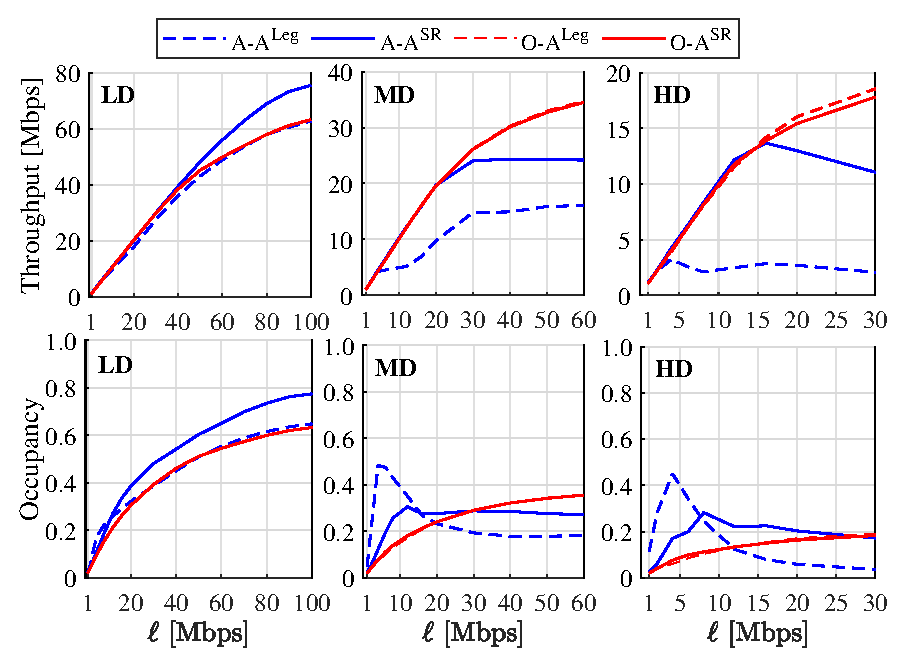
\includegraphics[width=0.6\textwidth]{img/throughput_occupancy.eps}
\end{figure}

\footnotesize
Throughput and channel occupancy experienced by WLAN$_A$ (A) and the other WLANs (O) in low (LD), medium (MD) and high density (HD) deployments. Each curve is named in the legend in the format X-A$^{\text{m}}$, where A$^{\text{m}}$ represents whether WLAN$_A$ uses spatial reuse (SR) or not (Leg).

\end{frame}

\subsection{}
\begin{frame}{Results (Delay)}
\begin{figure}
	\includegraphics[width=\textwidth]{img/cdf_delay.eps}
\end{figure}

	\footnotesize
	Empirical cumulative distribution function of the average packet delay experienced by WLAN$_A$. Different network densities and traffic loads are considered. Solid and dashed lines indicate whether WLAN$_A$ uses spatial reuse (SR) or not (Leg), respectively.
\end{frame}

%%% CONCLUSIONS
\section{Conclusions \& Future work}
\subsection{}
\begin{frame}{Conclusions \& Future work}
\begin{exampleblock}{Conclusions}
	\begin{itemize}
		\item We describe the OBSS/PD-based SR in IEEE 802.11ax
		\item Implementation of SR in Komondor $\rightarrow$ test novel algorithms
		\item Simulations show that SR enhances the performance (throughput and delay) of WLANs; specially, in dense scenarios
	\end{itemize}
\end{exampleblock}
\begin{alertblock}{Future work}
	\begin{itemize}
		\item Extend the analysis to scenarios where multiple WLANs apply SR
		\item Synergies of SR with other IEEE 802.11 features (scheduling, OFDMA, beamforming...)
		\item  Algorithm for setting up an \textit{optimal} OBSS/PD threshold
	\end{itemize}
\end{alertblock}
\end{frame}

%%% QUESTIONS
\appendix
\backupbegin
\section{}
\begin{frame}{Any questions?}
	\begin{figure}
		\includegraphics[width=\textwidth,height=0.4\textheight,keepaspectratio]{img/question_mark.png}
	\end{figure}
	\begin{center}	
		\footnotesize
		\textbf{Sergio Barrachina Mu\~noz, Ph.D. candidate}\\
		\textcolor{blue}{\textbf{sergio.barrachina@upf.edu}}\\
		Department of Communication and Information Technologies\\
		Universitat Pompeu Fabra (Barcelona, Spain)
	\end{center}
\end{frame}



% Backup slides here


\subsection{}
\begin{frame}{IEEE 802.11 SR operation}
	
	\begin{figure}
		\includegraphics[width=\textwidth,height=0.65\textheight,keepaspectratio]{img/sr_blocks.PNG}
	\end{figure}
	
	\footnotesize
	* Tutorial on 11ax SR: \textit{Wilhelmi et. al. ``Spatial Reuse in IEEE 802.11ax WLANs.'' preprint}
\end{frame}

\begin{frame}{OBSS/PD equation}
	Maximum OBSS/PD threshold:
	\begin{empheq}[box=\mymath]{equation*}
		\begin{align}\nonumber \text{OBSS/PD} \leq & \max\Big(\text{OBSS/PD}_{\min}, \min\big(\text{OBSS/PD}_{\max},\\ & \text{OBSS/PD}_{\min} + (\text{TX\_PWR}_{\text{ref}}-\text{TX\_PWR})\big)\Big) \nonumber \end{align}
	\end{empheq}
	Maximum transmit power:
	\begin{empheq}[box=\mymath]{equation*}
		\resizebox{.9\columnwidth}{!}{$\text{TX\_PWR}_{\max} = \text{TX\_PWR}_{\text{ref}} - (\text{OBSS/PD} -\text{OBSS/PD}_{\min})$}
		\nonumber
	\end{empheq}
\end{frame}



\backupend

\end{document}